\section{FAB-MAP 2.0}

\subsection{Introduction}
\begin{frame}{FAB-MAP 2.0}
    \begin{itemize}
        \item What happened after version 1.0 ?
    \end{itemize}
    \begin{quotation}
        We describe a formulation which preserves almost all the key features of our earlier model, but allows for the exploitation of the sparsity of visual word data to achieve large reductions in computation and memory requirements.~\cite{fabmap2011}
    \end{quotation}
    \begin{itemize}
        \item General intuition of the work in 2.0
    \end{itemize}
    \note[item]{Section: Fabmap 2}
    \note[item]{Read quotation}
    \note[item]{I will not go into details...}
    \note[item]{A lot of small changes}
    \note[item]{General intuition/main points.}
\end{frame}

\subsection{Modifications}
\begin{frame}
    \frametitle{Probabilistic Model}
    \begin{itemize}
        \item Sparse approximation
        \item Inverted index
        \item Appearance likelihood changed in two ways
            \begin{enumerate}
                \item Restrictions on the probabilities in the location models
                \item Data association
            \end{enumerate}
        \item Implementation in O(\#vocab)
    \end{itemize}
    \note[item]{Document is considered as a list of word identifiers, inverted index:mapping from words to documents.}
    \note[item]{Appearance likelihood was changed...to work with inverted index}
    \note[item]{Negative observations greatly outnumber positive ones, and are also generally less informative}
    \note[item]{Ignoring negatives yield bad results}
    \note[item]{*Single* probabilistic term for all observations of a place. Lead to some (negligible) information lost}
    \note[item]{Data association: sample-based instead of average appearance of a location (Location == set of samples.... Better suited for multi-modal)}
    \note[item]{They give the example of the open vs closed door}
    \note[item]{Complexity... because of CLT ~= O(1), worst case O(\#vocab)}
\end{frame}

\begin{frame}{Geometric Verification}
    \begin{center}
        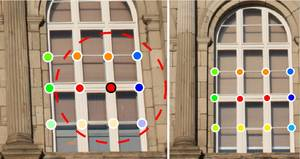
\includegraphics[width=0.8\textwidth]{./media/geo_verif.jpg}
    \end{center}
    \begin{itemize}
        \item Test on the 100 most likely samples
        \item Essential at large scale
    \end{itemize}
    \note[item]{Brief description of geometric verification}
    \note[item]{Do it on the best 100 samples}
    \note[item]{Also talk about Motion Model, but this is not new}
    \note[item]{Likely to be at one of the topologically adjacent locations}
    \note[item]{Used as a prior for the probabilistic model}
\end{frame}

\begin{frame}{K-Means}
    \begin{itemize}
        \item Approximation of the k-means algorithm \citet{kmeans}
        \item Fixed-radius incremental pre-clustering
        \item Cluster merging heuristic
        \item This boosted performance of the system
    \end{itemize}
    \note[item]{To maintain system performance at scale, they had to make some changes}
    \note[item]{Large density variations in feature space}
    \note[item]{After each k-means iteration, if any two cluster centers are closer than a fixed threshold, one of the two cluster centers is re-initialized to a random location.}
\end{frame}

\subsection{Results}
\begin{frame}{Results}
    \begin{columns}
        \begin{column}{0.4\textwidth}
            \begin{itemize}
                \item Validate on 1000~km dataset
                \item Ground thruth: GPS
                \item Same place < 40m
                    \begin{itemize}
                        \item 89\% < 5m
                        \item 98\% < 10m
                    \end{itemize}
            \end{itemize}
        \end{column}
        \begin{column}{0.6\textwidth}
            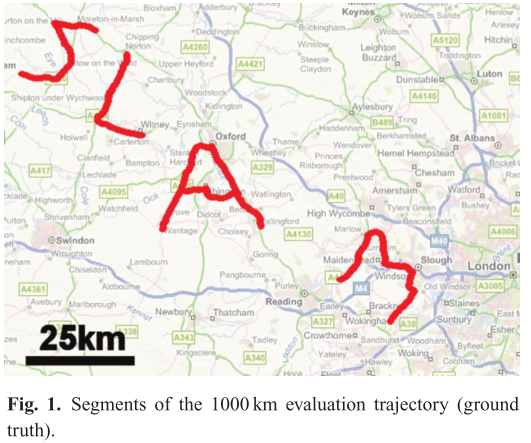
\includegraphics[width=1.0\textwidth]{./media/map_fabmap2.png}
        \end{column}
    \end{columns}
    \note[item]{Section: Results}
    \note[item]{Validate the work on a 1000km data set}
    \note[item]{Really aimed at large scale (other with 66km but they have the biggest)}
\end{frame}

\begin{frame}{Geometric Verification}
    \begin{center}
        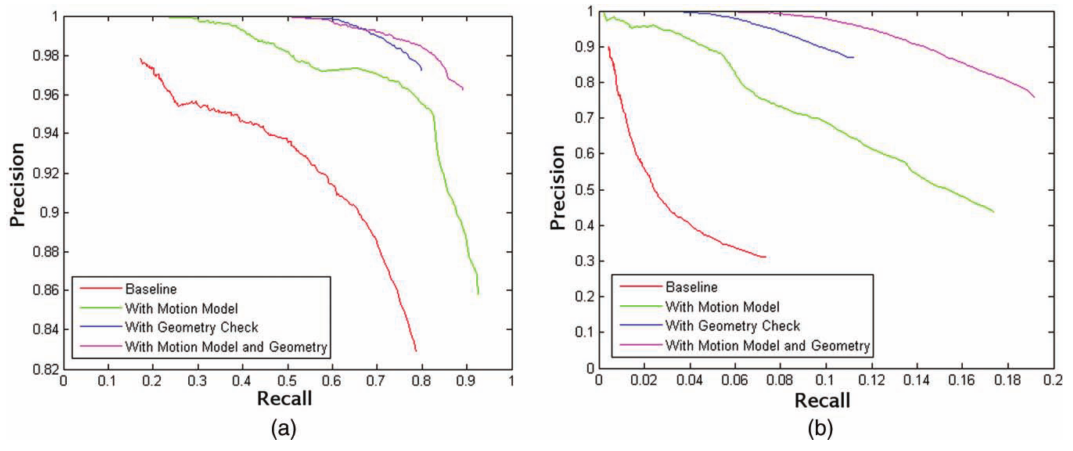
\includegraphics[width=1.0\textwidth]{./media/results_geo_verif.png}
    \end{center}
    \note[item]{Baseline refers to the system without the geometric check and with a uniform position prior at each timestep}
    \note[item]{Another important thing here is the value of the geometric verification}
\end{frame}

\begin{frame}{K-Means Words}
    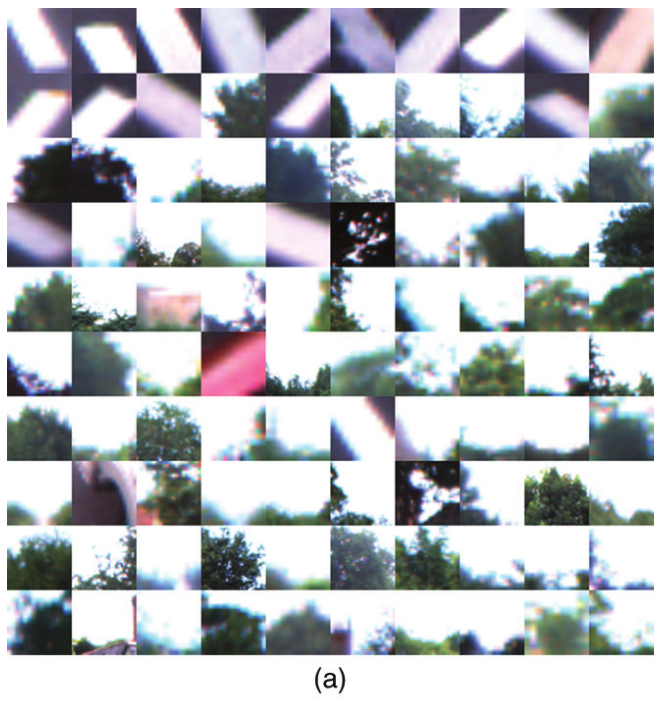
\includegraphics[width=0.5\textwidth]{./media/words_fabmap2a.png}
    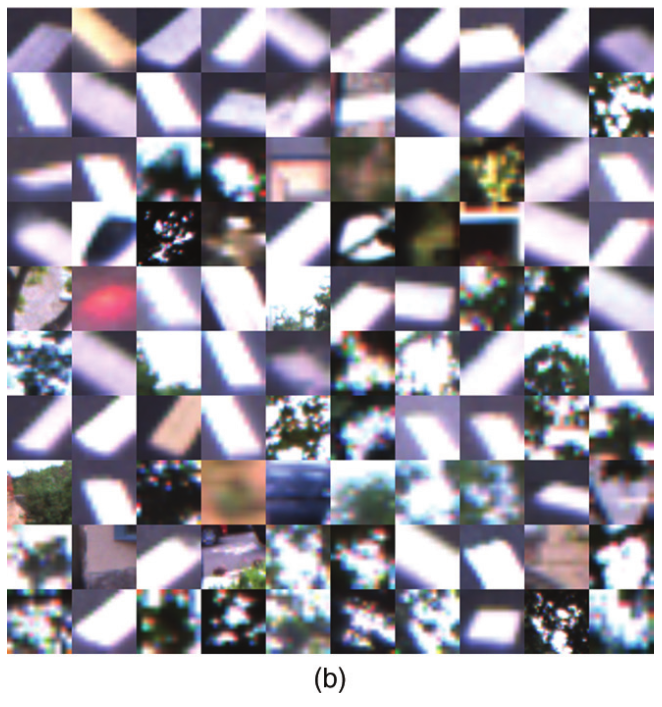
\includegraphics[width=0.5\textwidth]{./media/words_fabmap2b.png}
    \note[item]{Result changes for fixed-radius initialization}
    \note[item]{a) show words using the fixed radius initialization...}
    \note[item]{and b) is without change}
\end{frame}

\begin{frame}{K-Means}
    \begin{center}
        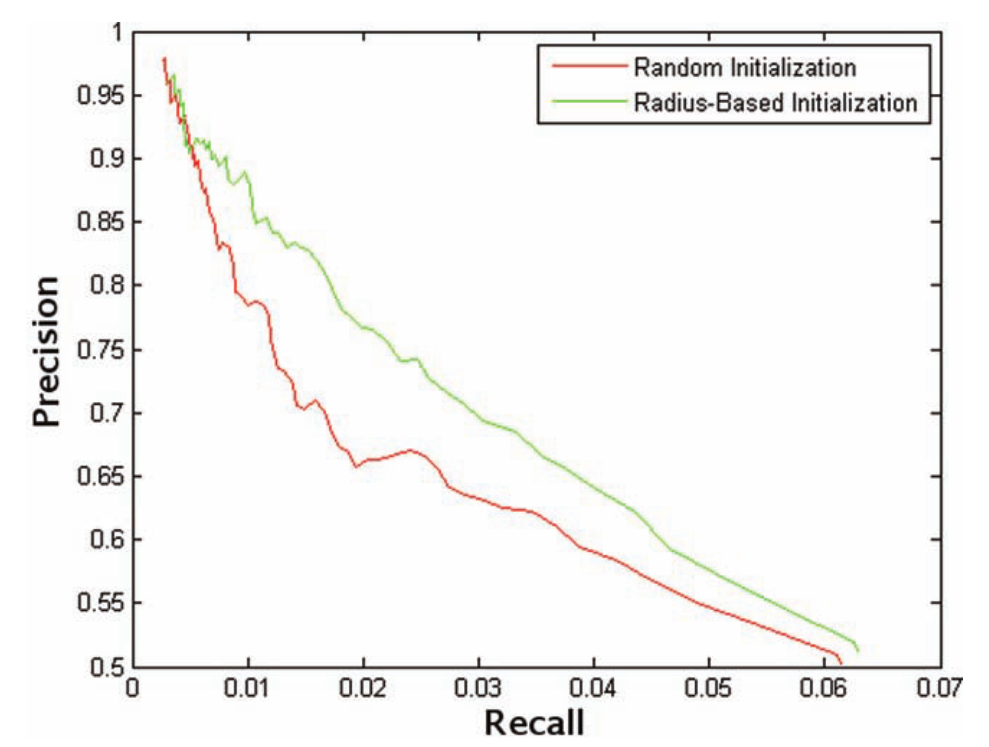
\includegraphics[width=0.7\textwidth]{./media/precision_recall_kmeans.png}
    \end{center}
    \note[item]{Not much to say except that the results are better}
    \note[item]{I just wonder why they show the curve when they want 100\% precision}
\end{frame}

\begin{frame}{Chow Liu and Naive Bayes}
    \begin{center}
        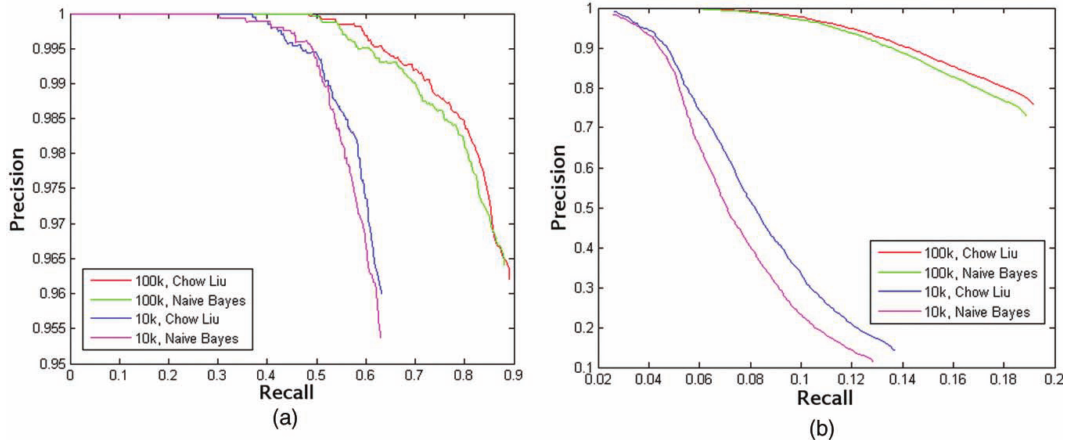
\includegraphics[width=1.0\textwidth]{./media/results2.png}
    \end{center}
    \note[item]{Finally, we also investigated the importance of learning the Chow Liu tree by comparing against a Naive Bayes formulation which neglects the cor- relations between words.}
    \note[item]{Maybe table 3, indicate that CL vs NB for 100\% precision}
\end{frame}

\begin{frame}{Comparison TF-IDF}
    \begin{center}
        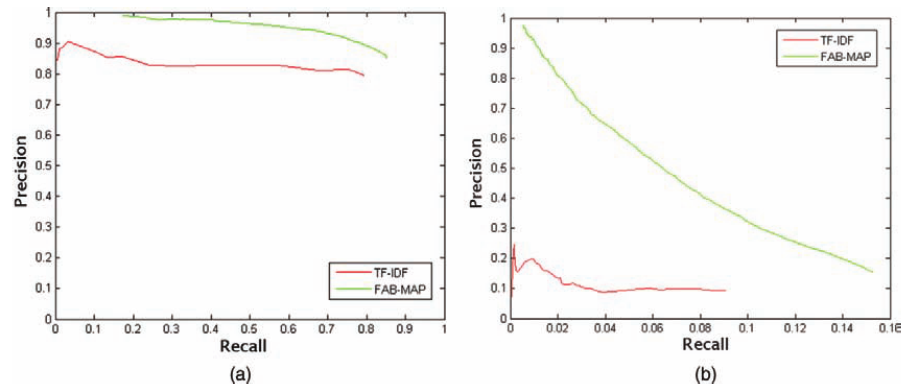
\includegraphics[width=1.0\textwidth]{./media/results_vs_tfidf.png}
    \end{center}
    \note[item]{Compared with tf-idf ranking measurements}
    \note[item]{Term-frequency inverse-document-frequency (tf-idf) is a standard ranking metric used in most existing visual search engines}
    \note[item]{We also demonstrate that the approach substantially outperforms the standard term-frequency inverse-document-frequency (tf-idf) ranking measure}
\end{frame}

\begin{frame}{Processing Time}
    \begin{itemize}
        \item 14ms filter update + geometric verification
        \item 423ms SURF
        \item 60ms quantization
        \item 4400 times faster than 1.0
    \end{itemize}
    \note[item]{Features are detected in raw sensory data, and these features are then quantized with respect to a vocabulary, yielding visual words.}
\end{frame}
